\documentclass[11pt,a4paper]{article}
\usepackage[utf8]{inputenc}
\usepackage[T1]{fontenc}
\usepackage{mathpazo}
\usepackage[margin=1.05in]{geometry}
\usepackage{amsmath,amssymb,amsthm,mathtools}
\usepackage{bm}
\usepackage{xcolor}
\usepackage[most]{tcolorbox}
\usepackage{enumitem}
\usepackage{booktabs}
\usepackage{caption}
\usepackage{tikz}
\usetikzlibrary{calc,arrows.meta,decorations.pathreplacing,positioning,shapes.geometric}
\usepackage{titlesec}
\usepackage{fancyhdr}
\usepackage{hyperref}
\usepackage[protrusion=true,expansion=false]{microtype}

\definecolor{accent}{HTML}{2c5282}
\definecolor{accent2}{HTML}{6b46c1}
\definecolor{good}{HTML}{2f855a}
\definecolor{bad}{HTML}{c53030}
\definecolor{neutral}{HTML}{4a5568}
\definecolor{paper}{HTML}{fafaf5}
\definecolor{goodfill}{HTML}{f0fdf4}
\definecolor{badfill}{HTML}{fef2f2}
\definecolor{keyfill}{HTML}{eff6ff}
\definecolor{idea}{HTML}{b45309}
\definecolor{ideafill}{HTML}{fffbeb}

\hypersetup{colorlinks=true, urlcolor=accent, linkcolor=accent, citecolor=accent}

\titleformat{\section}
  {\Large\bfseries\color{accent}}{\thesection}{0.7em}{}
\titleformat{\subsection}
  {\large\bfseries\color{accent}}{\thesubsection}{0.6em}{}
\titleformat{\subsubsection}
  {\normalsize\bfseries\color{accent2}}{\thesubsubsection}{0.5em}{}

\pagestyle{fancy}
\fancyhf{}
\fancyhead[L]{\small\itshape\color{neutral} JMVR triangular: derivation \& two bugs}
\fancyhead[R]{\small\color{neutral}\thepage}
\renewcommand{\headrulewidth}{0pt}

\newtcolorbox{keyresult}[1][]{enhanced, breakable, sharp corners,
  colback=keyfill, colframe=accent, boxrule=0pt, leftrule=3pt,
  fonttitle=\bfseries\color{accent}, title=#1,
  attach boxed title to top left={xshift=0.5em, yshift=-2mm},
  boxed title style={colback=keyfill, sharp corners, boxrule=0pt}}

\newtcolorbox{correctbox}[1][]{enhanced, breakable, sharp corners,
  colback=goodfill, colframe=good, boxrule=0pt, leftrule=3pt,
  fonttitle=\bfseries\color{good}, title=#1,
  attach boxed title to top left={xshift=0.5em, yshift=-2mm},
  boxed title style={colback=goodfill, sharp corners, boxrule=0pt}}

\newtcolorbox{buggybox}[1][]{enhanced, breakable, sharp corners,
  colback=badfill, colframe=bad, boxrule=0pt, leftrule=3pt,
  fonttitle=\bfseries\color{bad}, title=#1,
  attach boxed title to top left={xshift=0.5em, yshift=-2mm},
  boxed title style={colback=badfill, sharp corners, boxrule=0pt}}

\newtcolorbox{intuition}[1][Intuition]{enhanced, breakable, sharp corners,
  colback=ideafill, colframe=idea, boxrule=0pt, leftrule=3pt,
  fonttitle=\bfseries\itshape\color{idea}, title=#1,
  attach boxed title to top left={xshift=0.5em, yshift=-2mm},
  boxed title style={colback=ideafill, sharp corners, boxrule=0pt}}

\newcommand{\nn}{\nonumber \\}
\newcommand{\vk}{\mathbf{k}}
\newcommand{\vr}{\mathbf{r}}
\newcommand{\vn}{\mathbf{n}}
\newcommand{\vx}{\mathbf{x}}
\newcommand{\va}[1]{\mathbf{a}_{#1}}
\newcommand{\vb}[1]{\mathbf{b}_{#1}}
\newcommand{\veps}[1]{\hat{\mathbf{e}}_{#1}}
\newcommand{\vT}[1]{\mathbf{T}_{#1}}
\newcommand{\Ptilde}{\widetilde{P}}
\renewcommand{\d}{\mathrm{d}}

\begin{document}

% ===============================================================
% TITLE PAGE
% ===============================================================
\thispagestyle{empty}
\vspace*{0.7cm}
\begin{center}
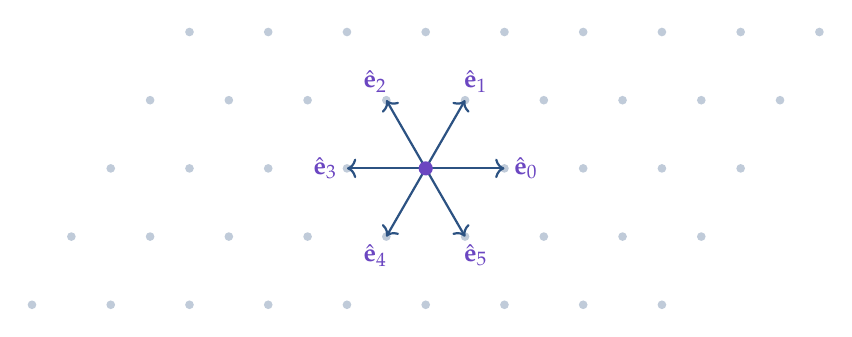
\begin{tikzpicture}[scale=0.5]
  \pgfmathsetmacro{\sq}{sqrt(3)}
  \foreach \i in {-4,...,4} {
    \foreach \j in {-2,...,2} {
      \pgfmathsetmacro{\x}{2*\i + \j}
      \pgfmathsetmacro{\y}{\sq*\j}
      \fill[accent!30] (\x,\y) circle (0.11);
    }
  }
  \foreach \dir/\lab in {0/{$\veps{0}$},60/{$\veps{1}$},120/{$\veps{2}$},180/{$\veps{3}$},240/{$\veps{4}$},300/{$\veps{5}$}} {
    \draw[->,thick,accent] (0,0) -- (\dir:2);
    \node[accent2,font=\small] at (\dir:2.55) {\lab};
  }
  \fill[accent2] (0,0) circle (0.18);
\end{tikzpicture}

\vspace{1cm}
{\Huge\bfseries\color{accent} The JMVR active random walker \\[2mm] on the triangular lattice}\\[6mm]
{\Large\itshape A complete derivation, two bugs, \\ and a verification protocol}\\[14mm]

{\large \textbf{P.\ Bisht} \;\,\small (TIFR Hyderabad)}\\[3mm]
{\small\itshape Notes for K.~Ramola\,---\,after the meeting of 4 May 2026}\\[12mm]

{\small 14 May 2026}\\[10mm]

\begin{tcolorbox}[enhanced, sharp corners, width=0.88\linewidth, colback=keyfill,
  colframe=accent, boxrule=0pt, leftrule=3pt, fonttitle=\bfseries\color{accent},
  title=Abstract]
\small
We derive, from first principles and with every algebraic step written out,
the master equation, the $6\times 6$ Bloch generator, and the
inverse-Fourier formula for the JMVR-style active random walker on the
triangular lattice with periodic boundary conditions. Two independent
errors in the {\sf{rtp\_tl\_2.nb}} notebook used in the unfinished
\emph{Confinement 2021} draft are identified and fixed:
\begin{enumerate}[label=(\roman*),leftmargin=*,itemsep=0pt]
\item a sign error in the chirality term of the coefficient $c_3$ of the
  Bloch matrix (master equation for director $m=2$);
\item a rectangular Fourier grid that violates the skew periodicity of the
  triangular torus, so the inverse-Fourier basis is not orthonormal on the
  discrete lattice.
\end{enumerate}
Either fix alone leaves the analytic $P(n_1, n_2, t)$ away from the
kinetic Monte Carlo result by a factor of order $10^2$ in RMS; both together
bring agreement to the Monte Carlo noise floor. Closed-form sanity checks
at $\vk = 0$ and in the achiral limit $\epsilon = 0$ are worked out
explicitly. The document is fully self-contained: notation is set up from
scratch and every formula is derived, not asserted.
\end{tcolorbox}
\end{center}
\vfill
\noindent {\footnotesize \color{neutral} TIFR Hyderabad \;\textbar\; DP1\,$\to$\,DP2 transition note}
\newpage
\setcounter{page}{1}

\tableofcontents
\vspace{1cm}

% ===============================================================
\section{Introduction and roadmap}\label{sec:intro}

\subsection{Why this calculation matters}\label{ssec:why}

The Jose-Mandal-Barma-Ramola (JMVR) active-walker model%
\footnote{Jose, Mandal, Barma, Ramola, \emph{Active random walks in one
and two dimensions}, Phys.\ Rev.\ E \textbf{105}, 064103 (2022);
\href{https://arxiv.org/abs/2202.02995}{arXiv:2202.02995}.} is the home
model of the Confinement-enhanced clustering programme at TIFR Hyderabad. The 2021 draft by Mandal, Barma,
and Ramola extended it to the 2D square lattice and outlined the
triangular extension in Section IV.B, but never completed it. The
notebook {\sf{rtp\_tl\_2.nb}} (D.~Mandal, 2019) was the working
implementation; it was abandoned because, in Kabir's own words at the 4
May 2026 meeting, ``I think Dipanjan implemented the boundary conditions
wrong.''

\subsection{What this document does}\label{ssec:what}

Two things, in order:
\begin{enumerate}[leftmargin=*]
\item \textbf{Derive everything from scratch.} Master equation, Fourier
  transform on the triangular torus, and the $6\times 6$ Bloch generator
  $M(\vk)$. Every algebraic step is shown.
\item \textbf{Diagnose and fix two bugs} in the 2019 notebook and Eq.~B11
  of the draft. Both fixes are needed; either alone leaves the theory
  off the kinetic Monte Carlo (KMC) ground truth by factors of 30--100$\times$.
\end{enumerate}

\subsection{Roadmap of the derivation}\label{ssec:roadmap}

\begin{center}
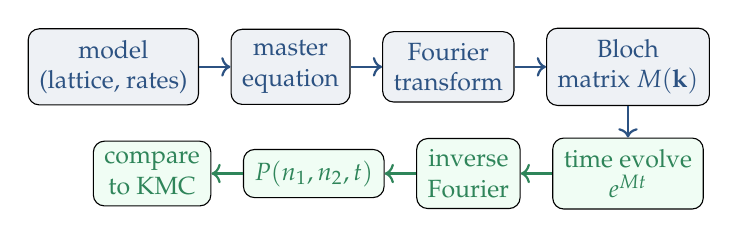
\begin{tikzpicture}[scale=1.0, node distance=4mm,
  every node/.style={font=\small, align=center, inner sep=4pt}]
\node[draw, rounded corners, fill=accent!8, text=accent] (model) {model\\(lattice, rates)};
\node[draw, rounded corners, fill=accent!8, text=accent, right=of model] (master) {master\\equation};
\node[draw, rounded corners, fill=accent!8, text=accent, right=of master] (fourier) {Fourier\\transform};
\node[draw, rounded corners, fill=accent!8, text=accent, right=of fourier] (bloch) {Bloch\\matrix $M(\vk)$};
\node[draw, rounded corners, fill=goodfill, text=good, below=of bloch] (solve) {time evolve\\$e^{Mt}$};
\node[draw, rounded corners, fill=goodfill, text=good, left=of solve] (invft) {inverse\\Fourier};
\node[draw, rounded corners, fill=goodfill, text=good, left=of invft] (Pxyt) {$P(n_1, n_2, t)$};
\node[draw, rounded corners, fill=goodfill, text=good, left=of Pxyt] (kmc) {compare\\to KMC};
\draw[->, accent, thick] (model) -- (master);
\draw[->, accent, thick] (master) -- (fourier);
\draw[->, accent, thick] (fourier) -- (bloch);
\draw[->, accent, thick] (bloch) -- (solve);
\draw[->, good, thick] (solve) -- (invft);
\draw[->, good, thick] (invft) -- (Pxyt);
\draw[->, good, thick] (Pxyt) -- (kmc);
\end{tikzpicture}\\[3mm]
{\footnotesize Sections \ref{sec:model}--\ref{sec:bloch} build the
analytic chain (blue); Sections \ref{sec:solving}--\ref{sec:verification}
evaluate and compare (green); Sections \ref{sec:c3-bug}, \ref{sec:pbc-bug}
locate the two bugs along this chain.}
\end{center}

\subsection{Notation reference}\label{ssec:notation}

\begin{center}\small
\renewcommand{\arraystretch}{1.18}
\begin{tabular}{ll}
\toprule
symbol & meaning \\
\midrule
$a, b$ & lattice basis parameters; $a = b = 1$ in {\sf{rtp\_tl\_2.nb}} \\
$\va{1}, \va{2}$ & primitive lattice vectors $= (2a, 0), (a, b)$ \\
$L$ & linear size of the torus ($L \times L$ unit cells) \\
$(n_1, n_2)$ & integer lattice indices, $\in \{0, \ldots, L-1\}^2$ on torus \\
$\vr(n_1, n_2)$ & Cartesian position, $= n_1 \va{1} + n_2 \va{2}$ \\
$m \in \{0,\ldots,5\}$ & director state (internal orientation) \\
$\veps{d}$ & Cartesian displacement to NN $d$, see Eq.~(\ref{eq:nn_cart}) \\
$\Delta(d)$ & integer-index displacement to NN $d$, see Eq.~(\ref{eq:nn_int}) \\
$\epsilon$ & translation chirality, $\epsilon \in [0, 1/6]$ \\
$\gamma$ & total rotation rate (sum of two $\gamma/2$ branches) \\
$P_m(n_1, n_2, t)$ & joint probability: at site $(n_1, n_2)$, director $m$, time $t$ \\
$\Ptilde_m(\vk, t)$ & Fourier transform of $P_m$ \\
$\vb{1}, \vb{2}$ & reciprocal lattice vectors, $\va{i}\cdot \vb{j} = 2\pi \delta_{ij}$ \\
$\vT{1}, \vT{2}$ & torus translation vectors, $= L \va{1}, L \va{2}$ \\
$M(\vk)$ & $6\times 6$ Bloch generator \\
$c_1, c_2, c_3$ & three independent diagonal entries of $M(\vk)$ \\
$B(\vk)$ & lattice-bulk dispersion (real, $m$-independent) \\
\bottomrule
\end{tabular}
\end{center}

% ===============================================================
\section{Physical picture: run, tumble, repeat}\label{sec:picture}

Before any algebra, here is what the model \emph{does}. A particle sits
at a lattice site carrying an internal arrow (the director $m$). At
exponentially-distributed waiting times it does one of two things:

\begin{enumerate}[leftmargin=*]
\item \textbf{Hop.} Most of the time, it hops to one of the six nearest
  neighbours. The hop is biased: with probability slightly above $1/6$
  it hops along its arrow (\emph{forward}); slightly below $1/6$ in the
  opposite direction (\emph{backward}); and exactly $1/6$ in each of the
  four perpendicular directions (\emph{sideways}). The bias is the
  chirality $\epsilon$.
\item \textbf{Rotate.} Less often (rate $\gamma$, with $\gamma \ll 1$),
  the arrow snaps by 60$^\circ$ to the left or right with equal
  probability. The new direction then governs subsequent hops.
\end{enumerate}

\begin{center}
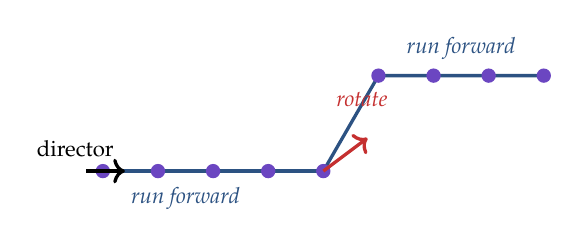
\begin{tikzpicture}[scale=0.7]
\pgfmathsetmacro{\sq}{sqrt(3)}
% Run path with rotation kink in the middle
\draw[very thick, accent] (0,0) -- (1,0) -- (2,0) -- (3,0) -- (4,0);
\draw[very thick, accent] (4,0) -- (5, \sq) -- (6, \sq) -- (7, \sq) -- (8, \sq);
\foreach \x/\y in {0/0, 1/0, 2/0, 3/0, 4/0, 5/\sq, 6/\sq, 7/\sq, 8/\sq} {
  \fill[accent2] (\x,\y) circle (0.13);
}
\draw[->, very thick, bad] (4,0) -- (4.8, 0.6); % rotation kink visualization
\node[bad, font=\footnotesize\itshape] at (4.7, 1.3) {rotate};
\node[accent, font=\footnotesize\itshape] at (1.5, -0.5) {run forward};
\node[accent, font=\footnotesize\itshape] at (6.5, \sq + 0.5) {run forward};
\draw[->, very thick] (-0.3, 0) -- (0.4, 0);
\node[font=\footnotesize] at (-0.5, 0.4) {director};
\end{tikzpicture}\\[2mm]
{\footnotesize A typical trajectory at small $\gamma$: long ballistic
runs along the current director, punctuated by rare 60$^\circ$ rotation
kinks. The shape of the time-$t$ probability density depends on whether
$\gamma t \ll 1$ (ballistic, hexagonal ring), $\gamma t \sim 1$
(diffusive-with-rotation crossover), or $\gamma t \gg 1$ (isotropic
diffusion with $D_{\rm eff} = \epsilon^2 / \gamma$).}
\end{center}

\begin{intuition}[Why these specific rates?]
The total translation rate is $1$ regardless of $\epsilon$: chirality
biases \emph{which} of the 6 NN the walker visits, not \emph{how often}
it hops. The total rotation rate is $\gamma$. These choices match the
JMVR 2022 paper's convention and make the achiral limit
$\epsilon \to 0$ a clean symmetric random walk.
\end{intuition}

% ===============================================================
\section{The model}\label{sec:model}

\subsection{The triangular Bravais lattice}\label{ssec:lattice}

The triangular Bravais lattice is generated by two primitive vectors
that make an angle of $60^\circ$ with each other. We use the
parametrization
\begin{equation}\label{eq:basis}
\va{1} \;=\; (2a, \, 0), \qquad \va{2} \;=\; (a, \, b),
\end{equation}
with $a, b > 0$. Two natural conventions appear:
\begin{itemize}[leftmargin=*]
\item \textbf{Algebraic} $a = b = 1$. Used in the Confinement 2021 draft
  and the notebook {\sf{rtp\_tl\_2.nb}}. Then $\va{1} = (2, 0)$ and
  $\va{2} = (1, 1)$; the nearest-neighbour Cartesian distances are $2$
  (for $\pm \va{1}$) and $\sqrt{2}$ (for the other four), so the lattice
  is \emph{not} geometrically isotropic in this convention.
\item \textbf{Isotropic} $a = 1$, $b = \sqrt{3}$. Then $\va{1} = (2, 0)$
  and $\va{2} = (1, \sqrt{3})$; all six nearest-neighbour displacements
  have equal Cartesian length~$2$.
\end{itemize}
\begin{keyresult}[Display-basis ambiguity, stated once and for all]
The choice of $(a, b)$ does \emph{not} affect any algebra below: the
lattice-coordinate probability $P(n_1, n_2, t)$ depends only on the
master-equation rates, which are parametrised by $\epsilon$ and $\gamma$
alone. $(a, b)$ enters only when we map integer lattice indices to
Cartesian positions in (\ref{eq:cartesian}) -- that is, when we
\emph{draw} the lattice or compute a Cartesian moment.
\end{keyresult}
\noindent We keep $a, b$ symbolic throughout the algebra. The
algebraic-convention values $a = b = 1$ match the Confinement-draft
formulas; the isotropic-convention values $a = 1, b = \sqrt{3}$ make our
figures geometrically faithful. Both produce identical $P(n_1, n_2, t)$.

A lattice site is labelled by integer indices $(n_1, n_2) \in \mathbb{Z}^2$
and sits at Cartesian position
\begin{equation}\label{eq:cartesian}
\vr(n_1, n_2) \;=\; n_1\, \va{1} + n_2 \, \va{2}
\;=\; \big(2 a n_1 + a n_2, \;\; b n_2\big).
\end{equation}

\subsection{Nearest neighbours}\label{ssec:nn}

Each site has six nearest neighbours, indexed $d \in \{0,\ldots,5\}$,
with Cartesian displacements
\begin{align}\label{eq:nn_cart}
\veps{0} &= +\va{1} = (+2a,\,0),
& \veps{1} &= +\va{2} = (+a,\,+b),
& \veps{2} &= -\va{1} + \va{2} = (-a,\,+b), \nn
\veps{3} &= -\va{1} = (-2a,\,0),
& \veps{4} &= -\va{2} = (-a,\,-b),
& \veps{5} &= +\va{1} - \va{2} = (+a,\,-b).
\end{align}
Equivalently, in lattice-index space:
\begin{align}\label{eq:nn_int}
\Delta(0) &= (+1,\,0),
& \Delta(1) &= (0,\,+1),
& \Delta(2) &= (-1,\,+1), \nn
\Delta(3) &= (-1,\,0),
& \Delta(4) &= (0,\,-1),
& \Delta(5) &= (+1,\,-1).
\end{align}

\vspace{3mm}

\begin{center}
\begin{tikzpicture}[scale=0.95]
  \pgfmathsetmacro{\sq}{sqrt(3)}
  \foreach \i in {-3,...,3} {
    \foreach \j in {-2,...,2} {
      \pgfmathsetmacro{\x}{2*\i + \j}
      \pgfmathsetmacro{\y}{\sq*\j}
      \fill[neutral!30] (\x,\y) circle (0.08);
    }
  }
  \foreach \i/\ang/\name/\dx/\dy in {0/0/$\veps{0}$/+1/0,
                                     1/60/$\veps{1}$/0/+1,
                                     2/120/$\veps{2}$/-1/+1,
                                     3/180/$\veps{3}$/-1/0,
                                     4/240/$\veps{4}$/0/-1,
                                     5/300/$\veps{5}$/+1/-1} {
    \draw[->, very thick, accent] (0,0) -- (\ang:2);
    \node[accent, font=\small\bfseries] at (\ang:2.45) {\name};
    \node[neutral!80, font=\scriptsize] at ({1.05*cos(\ang)}, {1.05*sin(\ang)+0.32}) {$\Delta=(\dx,\dy)$};
  }
  \fill[accent2] (0,0) circle (0.16);
  \node[anchor=south west, font=\small] at (0.1, 0.15) {site $(n_1, n_2)$};
  \draw[->, accent2, dashed, thick] (-5, -1.7) -- ($(-5, -1.7)+(2,0)$);
  \node[accent2, font=\small] at (-3.7, -1.95) {$\va{1}$};
  \draw[->, accent2, dashed, thick] (-5, -1.7) -- ($(-5, -1.7)+(1, \sq)$);
  \node[accent2, font=\small] at (-4.3, -0.5) {$\va{2}$};
\end{tikzpicture}
\captionof{figure}{The six nearest-neighbour displacements $\veps{d}$ on
the triangular lattice (isotropic visualization $b = \sqrt{3}\,a$).
$\Delta(d)$ is the corresponding shift in integer lattice indices.
Opposite NN form three pairs.}
\end{center}

\paragraph{Opposite-pair identity.} Direct inspection of (\ref{eq:nn_cart}) gives, for $d = 0, 1, 2$,
\begin{equation}\label{eq:opposite_id}
\boxed{\;\; \veps{d+3} \;=\; -\veps{d}, \;\;}
\end{equation}
with index arithmetic modulo $6$. This identity is used repeatedly below
to combine forward-backward pairs into a real cosine plus an imaginary
chirality sine.

\subsection{Torus geometry (periodic boundary conditions)}\label{ssec:torus}

The system is a finite torus of $L \times L$ unit cells:
\begin{equation}\label{eq:torus_id}
(n_1, n_2) \;\equiv\; (n_1 + L, n_2) \;\equiv\; (n_1, n_2 + L),
\end{equation}
with corresponding Cartesian translation vectors
\begin{equation}\label{eq:Tvecs}
\vT{1} \;=\; L\,\va{1} \;=\; (2 a L,\, 0), \qquad
\vT{2} \;=\; L\,\va{2} \;=\; (a L,\, b L).
\end{equation}

\begin{keyresult}[Skewness, in advance]
$\vT{2}$ has a nonzero $x$-component. Wrapping in the $n_2$ direction
shifts \emph{both} Cartesian coordinates, not just $y$. Forgetting this
skewness is the second bug we identify in Sec.~\ref{sec:pbc-bug}; it is
exactly the ``skew PBC trap'' Kabir drew during the meeting.
\end{keyresult}

\subsection{The walker and its transition rates}\label{ssec:walker}

A walker carries a lattice position $(n_1, n_2)$ and an internal
\emph{director} state $m \in \{0, \ldots, 5\}$ which picks one of the
six NN directions.

\paragraph{Translation.} From director $m$, the walker hops to NN site
$\vr + \veps{d}$ at rate
\begin{equation}\label{eq:trans_rates}
r_{\rm trans}(m \to d) \;=\;
\begin{cases}
\tfrac{1}{6} + \epsilon & d = m \quad \text{(forward)} \\[1mm]
\tfrac{1}{6} - \epsilon & d = (m+3) \bmod 6 \quad \text{(backward)} \\[1mm]
\tfrac{1}{6} & \text{otherwise (four sideways).}
\end{cases}
\end{equation}
\begin{equation}\label{eq:trans_total}
\sum_{d=0}^{5} r_{\rm trans}(m \to d) \;=\; \big(\tfrac{1}{6}+\epsilon\big) + \big(\tfrac{1}{6}-\epsilon\big) + 4 \cdot \tfrac{1}{6} \;=\; 1.
\end{equation}

\paragraph{Rotation.} The director switches by one step in each direction at rate $\gamma/2$:
\begin{equation}\label{eq:rot_rates}
r_{\rm rot}(m \to (m{\pm}1) \!\!\mod 6) \;=\; \tfrac{\gamma}{2},
\qquad \text{total rotation rate per state: } \gamma.
\end{equation}

\begin{center}
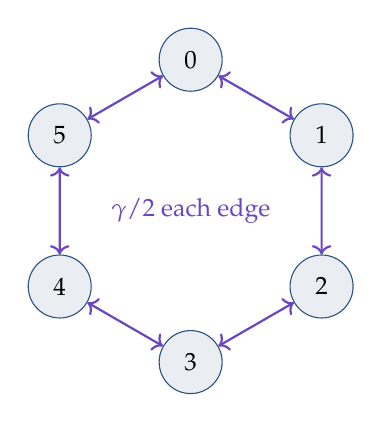
\begin{tikzpicture}[scale=1.2]
\foreach \i/\ang in {0/90, 1/30, 2/-30, 3/-90, 4/-150, 5/150} {
  \node[circle, draw=accent, fill=accent!10, minimum size=8mm, font=\small\bfseries] (n\i) at (\ang:1.6) {$\i$};
}
\foreach \i/\j in {0/1, 1/2, 2/3, 3/4, 4/5, 5/0} {
  \draw[<->, thick, accent2] (n\i) -- (n\j);
}
\node[accent2, font=\small] at (0, 0) {$\gamma/2$ each edge};
\end{tikzpicture}\\[2mm]
{\footnotesize The 6-director rotation graph. Each edge represents both
$m \to m \pm 1$ at rate $\gamma/2$; total rate $\gamma$ out of each
node.}
\end{center}

\paragraph{Total event rate per walker.} $1 + \gamma$. Inter-event waiting time is exponentially distributed.

% ===============================================================
\section{The master equation}\label{sec:master}

\subsection{Setup}\label{ssec:master-setup}

Let $P_m(n_1, n_2, t)$ denote the joint probability that at time $t$ the
walker sits at lattice site $(n_1, n_2)$ in director state $m$. The
probability obeys a continuous-time balance equation:
$\partial_t P_m = $ inflow $-$ outflow.

\paragraph{Outflow.} Total rate out of $(m; n_1, n_2)$:
\begin{equation}\label{eq:outflow}
r_{\rm out} \;=\; \sum_{d=0}^{5} r_{\rm trans}(m \to d) \;+\; \tfrac{\gamma}{2} + \tfrac{\gamma}{2} \;=\; 1 + \gamma,
\end{equation}
contributing $-(1+\gamma)P_m(n_1, n_2, t)$ to $\partial_t P_m$.

\paragraph{Inflow.} Two channels:
\begin{enumerate}[leftmargin=*,nosep]
\item \emph{Translation.} Walker in director $m$ at neighbouring site
  $(n_1, n_2) - \Delta(d)$ hops by $+\Delta(d)$ to arrive at
  $(n_1, n_2)$, at rate $r_{\rm trans}(m \to d)$:
  \begin{equation}\label{eq:inflow_trans}
  \sum_{d=0}^{5} r_{\rm trans}(m \to d)\; P_m\big(n_1 - \Delta_1(d),\, n_2 - \Delta_2(d),\, t\big).
  \end{equation}
\item \emph{Rotation.} Walker in adjacent director $m \pm 1$ at the same
  site rotates into director $m$ at rate $\gamma/2$ each:
  \begin{equation}\label{eq:inflow_rot}
  \tfrac{\gamma}{2}\, P_{m+1}(n_1, n_2, t) + \tfrac{\gamma}{2}\, P_{m-1}(n_1, n_2, t).
  \end{equation}
\end{enumerate}

\paragraph{General form.}
\begin{align}\label{eq:master_general}
\frac{\partial P_m(n_1, n_2, t)}{\partial t}
&= \sum_{d=0}^{5} r_{\rm trans}(m \to d)\; P_m\!\big(n_1{-}\Delta_1(d),\, n_2{-}\Delta_2(d),\, t\big) \nn
&\quad + \tfrac{\gamma}{2} P_{m+1}(n_1, n_2, t) + \tfrac{\gamma}{2} P_{m-1}(n_1, n_2, t) \nn
&\quad - (1 + \gamma) P_m(n_1, n_2, t).
\end{align}

\begin{intuition}[Why ``inflow from $(n_1, n_2) - \Delta(d)$''?]
The walker at $(n_1, n_2) - \Delta(d)$ hops by $+\Delta(d)$ to arrive at
$(n_1, n_2)$. So we are tracking who \emph{lands here} this instant,
which is who was \emph{one displacement away} and hopped here. The
minus sign in $-\Delta(d)$ is exactly the standard ``backwards advection''
sign in lattice master equations.
\end{intuition}

\subsection{Explicit form for $m = 0$}\label{ssec:master-m0}

Director $m = 0$: forward $\veps{0}$, backward $\veps{3}$. Substituting:
\begin{align}\label{eq:master_m0}
\frac{\partial P_0(n_1, n_2, t)}{\partial t}
&= \big(\tfrac{1}{6} + \epsilon\big)\, P_0(n_1 - 1, n_2,\, t) \nn
&\quad + \big(\tfrac{1}{6} - \epsilon\big)\, P_0(n_1 + 1, n_2,\, t) \nn
&\quad + \tfrac{1}{6}\, P_0(n_1, n_2 - 1, t) + \tfrac{1}{6}\, P_0(n_1, n_2 + 1, t) \nn
&\quad + \tfrac{1}{6}\, P_0(n_1 + 1, n_2 - 1, t) + \tfrac{1}{6}\, P_0(n_1 - 1, n_2 + 1, t) \nn
&\quad + \tfrac{\gamma}{2} P_1(n_1, n_2, t) + \tfrac{\gamma}{2} P_5(n_1, n_2, t) \nn
&\quad - (1 + \gamma) P_0(n_1, n_2, t).
\end{align}

\subsection{Explicit form for $m = 2$ (the buggy director)}\label{ssec:master-m2}

Director $m = 2$: forward $\veps{2} = (-a, b)$, backward $\veps{5} = (+a, -b)$.
From (\ref{eq:nn_int}), $\Delta(2) = (-1, 1)$ and $\Delta(5) = (1, -1)$:
\begin{align}\label{eq:master_m2}
\frac{\partial P_2(n_1, n_2, t)}{\partial t}
&= \big(\tfrac{1}{6} + \epsilon\big)\, P_2(n_1 + 1, n_2 - 1, t) \nn
&\quad + \big(\tfrac{1}{6} - \epsilon\big)\, P_2(n_1 - 1, n_2 + 1, t) \nn
&\quad + \tfrac{1}{6}\, P_2(n_1 - 1, n_2, t) + \tfrac{1}{6}\, P_2(n_1 + 1, n_2, t) \nn
&\quad + \tfrac{1}{6}\, P_2(n_1, n_2 - 1, t) + \tfrac{1}{6}\, P_2(n_1, n_2 + 1, t) \nn
&\quad + \tfrac{\gamma}{2} P_3(n_1, n_2, t) + \tfrac{\gamma}{2} P_1(n_1, n_2, t) \nn
&\quad - (1 + \gamma) P_2(n_1, n_2, t).
\end{align}
\textbf{This equation's Fourier transform gives the diagonal entry $c_3$
of the Bloch matrix} -- the source of the sign-error analysis in
Sec.~\ref{sec:c3-bug}.

\subsection{Probability conservation}\label{ssec:prob-conservation}

Summing (\ref{eq:master_general}) over $m$ at a fixed site, the
rotation contributions cancel pairwise (each $\gamma/2$ inflow into $m$
from $m \pm 1$ is exactly cancelled by the corresponding outflow from
$m \pm 1$ into $m$). The translation contributions sum to a discrete
divergence; summing further over all $(n_1, n_2)$ on the torus yields
zero. Hence the total probability $\sum_{n_1, n_2, m} P_m = 1$ is preserved.

% ===============================================================
\section{Fourier transform on the triangular torus}\label{sec:fourier}

\subsection{Reciprocal lattice}\label{ssec:reciprocal}

The reciprocal lattice basis $\{\vb{1}, \vb{2}\}$ is determined by the
duality relations
\begin{equation}\label{eq:reciprocal_def}
\va{i} \cdot \vb{j} \;=\; 2\pi\, \delta_{ij}.
\end{equation}
Writing $\vb{1} = (b_{1x}, b_{1y})$ and using
$\va{1} = (2a, 0), \va{2} = (a, b)$:
\[
\va{1} \cdot \vb{1} = 2a\, b_{1x} = 2\pi \implies b_{1x} = \pi/a, \quad
\va{2} \cdot \vb{1} = a\, b_{1x} + b\, b_{1y} = 0 \implies b_{1y} = -\pi/b.
\]
Similarly for $\vb{2}$:
\[
\va{1} \cdot \vb{2} = 2a\, b_{2x} = 0 \implies b_{2x} = 0, \quad
\va{2} \cdot \vb{2} = b\, b_{2y} = 2\pi \implies b_{2y} = 2\pi/b.
\]
\begin{equation}\label{eq:reciprocal_vecs}
\boxed{\;\;
\vb{1} \;=\; \Big(\tfrac{\pi}{a},\; -\tfrac{\pi}{b}\Big), \qquad
\vb{2} \;=\; \Big(0,\;\tfrac{2\pi}{b}\Big).
\;\;}
\end{equation}
$\vb{1}$ has a nonzero $y$-component: the Fourier-space mirror of the
real-space skewness in $\vT{2}$.

\subsection{Allowed wavevectors on the torus}\label{ssec:k-allowed}

For $\vk$ to give a torus-compatible plane wave $e^{i \vk \cdot \vr}$:
\begin{equation}\label{eq:torus_compatible}
\vk \cdot \vT{1} \;\in\; 2\pi\, \mathbb{Z}, \qquad
\vk \cdot \vT{2} \;\in\; 2\pi\, \mathbb{Z}.
\end{equation}
The $L^2$ inequivalent wavevectors are
\begin{equation}\label{eq:k_lattice}
\vk(m_1, m_2) \;=\; \frac{m_1}{L}\,\vb{1} + \frac{m_2}{L}\,\vb{2},
\qquad m_1, m_2 \in \{0, 1, \ldots, L-1\}.
\end{equation}
Substituting (\ref{eq:reciprocal_vecs}):
\begin{align}\label{eq:k_components}
k_x(m_1, m_2) &= \tfrac{m_1}{L}\cdot\tfrac{\pi}{a} + 0 = \tfrac{\pi m_1}{a L}, \nn
k_y(m_1, m_2) &= \tfrac{m_1}{L}(-\tfrac{\pi}{b}) + \tfrac{m_2}{L}\cdot\tfrac{2\pi}{b} = \tfrac{\pi(2 m_2 - m_1)}{b L}.
\end{align}

\begin{correctbox}[The sheared k-grid (the CORRECT grid for the triangular torus)]
\begin{equation}\label{eq:k_shear}
k_x \;=\; \frac{\pi\, m_1}{a L}, \qquad
k_y \;=\; \frac{\pi(2 m_2 - m_1)}{b L},
\qquad m_1, m_2 \in \{0, 1, \ldots, L-1\}.
\end{equation}
\end{correctbox}

\subsubsection{The hexagonal Brillouin zone}\label{ssec:bz}

In the isotropic convention ($b = \sqrt{3} a$), the reciprocal lattice
of the triangular Bravais lattice is itself triangular (rotated by
$30^\circ$), and its first Brillouin zone is a regular hexagon. The
high-symmetry points are $\Gamma$ (zone centre), $M$ (midpoint of zone
edge), and $K$ (zone corner):
\begin{center}
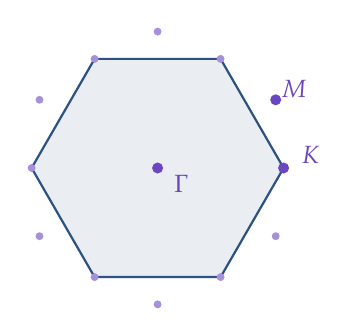
\begin{tikzpicture}[scale=1.0]
\pgfmathsetmacro{\sq}{sqrt(3)}
% Hexagonal BZ
\draw[thick, accent, fill=accent!10] (0:1.6) -- (60:1.6) -- (120:1.6) -- (180:1.6) -- (240:1.6) -- (300:1.6) -- cycle;
\fill[accent2] (0,0) circle (0.07);
\node[accent2, font=\small] at (0.3, -0.2) {$\Gamma$};
\fill[accent2] (30:\sq) circle (0.07);
\node[accent2, font=\small] at (30:2.0) {$M$};
\fill[accent2] (0:1.6) circle (0.07);
\node[accent2, font=\small] at (5:1.95) {$K$};
\foreach \ang in {60, 120, 180, 240, 300} {
  \fill[accent2!60] (\ang:1.6) circle (0.05);
}
\foreach \ang in {90, 150, 210, 270, 330} {
  \fill[accent2!60] ({\ang}:\sq) circle (0.05);
}
\end{tikzpicture}\\[1mm]
{\footnotesize First Brillouin zone of the triangular lattice (hexagon),
with high-symmetry points $\Gamma$, $M$, $K$. Our discrete sheared grid
samples this hexagon at $L^2$ points.}
\end{center}

\subsection{The Cartesian-to-index simplification}\label{ssec:cart_simplify}

Using (\ref{eq:cartesian}) and (\ref{eq:k_components}):
\begin{align}
\vk \cdot \vr(n_1, n_2)
&= k_x(2 a n_1 + a n_2) + k_y(b n_2) \nn
&= \frac{\pi m_1}{a L}(2 a n_1 + a n_2) + \frac{\pi(2 m_2 - m_1)}{b L}(b n_2) \nn
&= \frac{2\pi m_1 n_1}{L} + \frac{\pi m_1 n_2}{L} + \frac{\pi(2 m_2 - m_1) n_2}{L} \nn
&= \frac{2\pi m_1 n_1}{L} + \frac{2\pi m_2 n_2}{L} \nn
&= \boxed{\;\frac{2\pi(m_1 n_1 + m_2 n_2)}{L}\;}.
\label{eq:k_dot_r_clean}
\end{align}
The sheared grid is precisely the grid that makes the discrete Fourier
basis orthonormal on the $L \times L$ lattice in integer indices.

\subsection{The discrete Fourier pair}\label{ssec:dft}

\begin{equation}\label{eq:fft_pair}
\Ptilde_m(\vk, t) \;=\; \sum_{n_1, n_2 = 0}^{L-1} e^{\,i \vk \cdot \vr(n_1, n_2)} P_m(n_1, n_2, t),
\end{equation}
\begin{equation}\label{eq:ifft}
P_m(n_1, n_2, t) \;=\; \frac{1}{L^2}\sum_{\vk} e^{\,-i \vk \cdot \vr(n_1, n_2)}\, \Ptilde_m(\vk, t),
\end{equation}
with the sum in (\ref{eq:ifft}) over the $L^2$ sheared wavevectors.
Orthogonality follows from (\ref{eq:k_dot_r_clean}).

\subsection{Transforming the master equation term by term}\label{ssec:transform-stepwise}

Apply $\sum_{n_1, n_2} e^{i \vk \cdot \vr(n_1, n_2)}$ to (\ref{eq:master_general}). LHS gives $\partial_t \Ptilde_m(\vk, t)$.

\paragraph{Translation-in terms.} Change dummy index
$(n_1', n_2') = (n_1 - \Delta_1(d), n_2 - \Delta_2(d))$; then
$\vr(n_1, n_2) = \vr(n_1', n_2') + \veps{d}$ and on the torus the sum
ranges over the same set:
\begin{align}\label{eq:shift_step}
\sum_{n_1, n_2}\!\! e^{\,i \vk \cdot \vr(n_1, n_2)}\, P_m\!\big(n_1{-}\Delta_1(d), n_2{-}\Delta_2(d), t\big)
&= \sum_{n_1', n_2'}\!\! e^{\,i \vk \cdot (\vr(n_1', n_2') + \veps{d})}\, P_m(n_1', n_2', t) \nn
&= e^{\,i \vk \cdot \veps{d}}\, \Ptilde_m(\vk, t).
\end{align}
Applying to each of the six translation contributions in (\ref{eq:master_general}):
\begin{align}
\sum_{d=0}^{5} r_{\rm trans}(m{\to}d)\, e^{i \vk \cdot \veps{d}} \Ptilde_m(\vk, t)
&= \big(\tfrac{1}{6}{+}\epsilon\big) e^{i \vk \cdot \veps{m}} \Ptilde_m + \big(\tfrac{1}{6}{-}\epsilon\big) e^{i \vk \cdot \veps{m+3}} \Ptilde_m \nn
&\quad + \tfrac{1}{6}\!\!\!\!\sum_{d \notin \{m, m+3\}}\!\!\!\! e^{i \vk \cdot \veps{d}} \Ptilde_m.
\label{eq:trans_in_kspace}
\end{align}

\paragraph{Rotation-in terms.} Local in space, transform trivially:
$\tfrac{\gamma}{2} \Ptilde_{m+1} + \tfrac{\gamma}{2} \Ptilde_{m-1}$.

\paragraph{Outflow.} Trivial: $-(1 + \gamma) \Ptilde_m(\vk, t)$.

\paragraph{The Fourier-space master equation.}
\begin{correctbox}[Bloch-form master equation]
\begin{equation}\label{eq:master_k}
\frac{\partial \Ptilde_m(\vk, t)}{\partial t}
\;=\; \Big[\sum_{d=0}^{5} r_{\rm trans}(m \to d)\, e^{\,i\vk \cdot \veps{d}} - (1 + \gamma)\Big] \Ptilde_m
\;+\; \tfrac{\gamma}{2}\Ptilde_{m+1} + \tfrac{\gamma}{2}\Ptilde_{m-1}.
\end{equation}
\end{correctbox}

% ===============================================================
\section{The $6 \times 6$ Bloch matrix $M(\vk)$}\label{sec:bloch}

\subsection{Defining $M(\vk)$}\label{ssec:Mk_def}

Write (\ref{eq:master_k}) as
\[
\frac{\partial}{\partial t}\!\begin{pmatrix} \Ptilde_0 \\ \vdots \\ \Ptilde_5 \end{pmatrix}
= M(\vk) \begin{pmatrix} \Ptilde_0 \\ \vdots \\ \Ptilde_5 \end{pmatrix},
\]
with entries
\begin{align}\label{eq:Mk_entries}
M_{m,m}(\vk) &= \sum_{d=0}^{5} r_{\rm trans}(m \to d)\, e^{\,i\vk\cdot\veps{d}} - (1+\gamma), \nn
M_{m,\, m\pm 1 \bmod 6}(\vk) &= \tfrac{\gamma}{2}, \nn
M_{m, m'}(\vk) &= 0 \quad \text{otherwise.}
\end{align}

\subsection{Diagonal: forward-backward pair}\label{ssec:diag_fb}

Group the six terms in $M_{m,m}$ into three opposite pairs using
$\veps{m+3} = -\veps{m}$. For the forward-backward pair:
\begin{align}\label{eq:fb_pair_step}
&\big(\tfrac{1}{6}+\epsilon\big) e^{\,i\vk\cdot\veps{m}} + \big(\tfrac{1}{6}-\epsilon\big) e^{\,-i\vk\cdot\veps{m}} \nn
&\quad = \tfrac{1}{6}\big[e^{\,i\vk\cdot\veps{m}} + e^{\,-i\vk\cdot\veps{m}}\big] + \epsilon\big[e^{\,i\vk\cdot\veps{m}} - e^{\,-i\vk\cdot\veps{m}}\big] \nn
&\quad = \tfrac{1}{3}\cos(\vk\cdot\veps{m}) + 2 i \epsilon\, \sin(\vk\cdot\veps{m}).
\end{align}

\begin{intuition}[Why is the chirality term imaginary?]
The cosine piece is symmetric in $\vk \to -\vk$: it comes from the
symmetric part of the rates ($1/6$ in each direction). The sine piece is
antisymmetric in $\vk \to -\vk$: it comes from the asymmetric part of
the rates (the $\pm \epsilon$ forward-bias). Because $M$ has real
entries in real space (it's a generator of a Markov process), its
Fourier transform satisfies $M(-\vk) = M(\vk)^*$, which is precisely the
statement that the sine piece is imaginary.
\end{intuition}

\subsection{Diagonal: sideways pairs}\label{ssec:diag_side}

For each sideways pair $\{\veps{d}, \veps{d+3}\}$ (both at rate $1/6$):
\begin{equation}\label{eq:side_pair_step}
\tfrac{1}{6}\big[e^{\,i\vk\cdot\veps{d}} + e^{\,-i\vk\cdot\veps{d}}\big]
\;=\; \tfrac{1}{3}\cos(\vk\cdot\veps{d}).
\end{equation}

\subsection{The bulk term $B(\vk)$ is $m$-independent}\label{ssec:bulk_indep}

Summing the cosine contributions from all three pairs:
\begin{equation}\label{eq:bulk}
\boxed{\;\;
B(\vk) \;\equiv\; \tfrac{1}{3}\big[\cos(\vk\cdot\veps{0}) + \cos(\vk\cdot\veps{1}) + \cos(\vk\cdot\veps{2})\big].
\;\;}
\end{equation}

\subsection{Putting together the diagonal entry}\label{ssec:diag_total}

\begin{correctbox}[Diagonal entry of the Bloch matrix]
\begin{equation}\label{eq:diag_full}
M_{m,m}(\vk) \;=\; B(\vk) \;-\; 1 \;-\; \gamma \;+\; 2 i \epsilon \, \sin(\vk \cdot \veps{m}).
\end{equation}
\end{correctbox}

\subsection{Conjugation pairing of the diagonal entries}\label{ssec:conjugation}

Apply (\ref{eq:diag_full}) at $m \mapsto m + 3$ using $\veps{m+3} = -\veps{m}$ and $\sin(-X) = -\sin(X)$:
\begin{align}
M_{m+3, m+3}(\vk) &= B - 1 - \gamma + 2 i \epsilon \sin(\vk \cdot \veps{m+3}) \nn
&= B - 1 - \gamma - 2 i \epsilon \sin(\vk \cdot \veps{m}) \nn
&= \big[M_{m, m}(\vk)\big]^{*}.
\label{eq:conjugation_pair}
\end{align}
Pairs: $(M_{0,0}, M_{3,3})$, $(M_{1,1}, M_{4,4})$, $(M_{2,2}, M_{5,5})$.

\subsection{Naming convention: $c_1, c_2, c_3$}\label{ssec:cnames}
\[
c_1 \equiv M_{0,0}, \qquad c_2 \equiv M_{1,1}, \qquad c_3 \equiv M_{2,2},
\]
with $M_{3,3} = c_1^*, M_{4,4} = c_2^*, M_{5,5} = c_3^*$.

\subsection{Explicit form of $c_1, c_2, c_3$}\label{ssec:c_explicit}

Three NN displacements (\ref{eq:nn_cart}):
\[
\veps{0} = (+2a, 0), \qquad \veps{1} = (+a, +b), \qquad \veps{2} = (-a, +b).
\]
The bulk:
\begin{align}\label{eq:bulk_explicit}
B(\vk) &= \tfrac{1}{3}\big[\cos(2 a k_1) + \cos(a k_1 + b k_2) + \cos(-a k_1 + b k_2)\big] \nn
&= \tfrac{1}{3}\big[\cos(2 a k_1) + \cos(a k_1 + b k_2) + \cos(a k_1 - b k_2)\big].
\end{align}
The chirality terms:
\begin{align}
2 i \epsilon \sin(\vk \cdot \veps{0}) &= 2 i \epsilon \sin(2 a k_1), \\
2 i \epsilon \sin(\vk \cdot \veps{1}) &= 2 i \epsilon \sin(a k_1 + b k_2), \\
2 i \epsilon \sin(\vk \cdot \veps{2}) &= 2 i \epsilon \sin(-a k_1 + b k_2) \;=\; -2 i \epsilon \sin(a k_1 - b k_2).
\label{eq:chirality_m2}
\end{align}
The last line uses $\sin(-X) = -\sin(X)$ and is where the $\textbf{minus}$ in $c_3$ originates.

\begin{correctbox}[Correct diagonal entries]
\begin{align}\label{eq:c_final}
c_1 &= B(\vk) - 1 - \gamma + 2 i \epsilon \sin(2 a k_1), \nn
c_2 &= B(\vk) - 1 - \gamma + 2 i \epsilon \sin(a k_1 + b k_2), \nn
c_3 &= B(\vk) - 1 - \gamma \;\mathbf{-}\; 2 i \epsilon \sin(a k_1 - b k_2).
\end{align}
\end{correctbox}

\subsection{The full matrix}\label{ssec:Mk_full}

\begin{equation}\label{eq:Mk_explicit}
M(\vk) \;=\;
\begin{pmatrix}
c_1 & \gamma/2 & 0 & 0 & 0 & \gamma/2 \\
\gamma/2 & c_2 & \gamma/2 & 0 & 0 & 0 \\
0 & \gamma/2 & c_3 & \gamma/2 & 0 & 0 \\
0 & 0 & \gamma/2 & c_1^* & \gamma/2 & 0 \\
0 & 0 & 0 & \gamma/2 & c_2^* & \gamma/2 \\
\gamma/2 & 0 & 0 & 0 & \gamma/2 & c_3^*
\end{pmatrix}.
\end{equation}

% ===============================================================
\section{Closed-form check: $M(\vk = 0)$}\label{sec:k0-check}

A useful and complete cross-check is to compute the spectrum of $M$ at
$\vk = 0$ analytically. At $\vk = 0$, every $\sin$ vanishes, every
$\cos$ becomes $1$, so $B(0) = 1$ and the diagonal entries become
$-\gamma$. The matrix reduces to
\begin{equation}\label{eq:M_zero}
M(0) \;=\; \tfrac{\gamma}{2} C - \gamma I,
\end{equation}
where $C$ is the adjacency matrix of the 6-cycle (1s on the
$(m, m\pm 1) \bmod 6$ off-diagonals, 0 elsewhere) and $I$ is the
identity. Eigenvalues of $C$ are well-known:
$\lambda_n^{(C)} = 2\cos(2\pi n / 6) = 2\cos(\pi n/3)$ for $n = 0,\ldots,5$, i.e.,
$\{2, 1, -1, -2, -1, 1\}$. Hence
\begin{equation}\label{eq:M0_spectrum}
\boxed{\;\;\mathrm{spec}\,M(0) \;=\; \big\{0,\; -\tfrac{\gamma}{2},\; -\tfrac{3\gamma}{2},\; -2\gamma,\; -\tfrac{3\gamma}{2},\; -\tfrac{\gamma}{2}\big\}.\;\;}
\end{equation}

\begin{intuition}[What this means physically]
$\lambda = 0$ is the stationary mode -- the uniform distribution over
directors. The next-to-zero modes at $-\gamma/2$ are the slowest
relaxation channels (the dipole modes of director relaxation); $-2\gamma$
is the fastest, corresponding to the alternating pattern around the
6-cycle. All eigenvalues are real and non-positive, confirming that
$M(0)$ generates a relaxing Markov dynamics. The buggy and corrected
$c_3$ give the same spectrum at $\vk = 0$ because the chirality vanishes
there.
\end{intuition}

% ===============================================================
\section{Closed-form check: the achiral limit $\epsilon = 0$}\label{sec:eps0-check}

At $\epsilon = 0$ the chirality term vanishes identically. The diagonal
entries collapse to
\begin{equation}\label{eq:diag_eps0}
M_{m,m}(\vk)\big|_{\epsilon = 0} \;=\; B(\vk) - 1 - \gamma,
\end{equation}
the same for all $m$. The matrix becomes $M(\vk) = (B(\vk) - 1 - \gamma) I + \tfrac{\gamma}{2} C$,
diagonalized by the same Fourier basis as the 6-cycle. Eigenvalues:
\begin{equation}\label{eq:M_eps0_spec}
\lambda_n(\vk) = B(\vk) - 1 - \gamma + \gamma \cos(\pi n/3), \quad n = 0,\ldots,5.
\end{equation}
The $n = 0$ Perron eigenvalue is
\begin{equation}\label{eq:perron_eps0}
\lambda_0(\vk) \;=\; B(\vk) - 1.
\end{equation}
Summing $\lambda_0 \Ptilde_0$ over all $\vk$ and inverse-Fourier-transforming
gives the standard symmetric-walker propagator on the triangular lattice
-- exactly as expected, with no chirality.

\begin{intuition}[Sanity]
The achiral limit recovers the textbook symmetric continuous-time random
walk on the triangular lattice with hopping rate $1/6$ per direction.
Any candidate generator that fails to do this is wrong. Both the buggy
and corrected $c_3$ satisfy this limit (since the buggy term vanishes at
$\epsilon = 0$), so it is not by itself diagnostic.
\end{intuition}

% ===============================================================
\section{Bug 1: the $c_3$ sign error}\label{sec:c3-bug}

\subsection{What the Confinement draft and {\sf{rtp\_tl\_2.nb}} state}\label{ssec:dipanjan-c3}

\begin{buggybox}[Draft Eq.~B11 / notebook (BUGGY)]
\begin{equation}\label{eq:c3_dipanjan}
c_3^{\rm (draft)} \;=\; B(\vk) - 1 - \gamma \;\mathbf{+}\; 2 i \epsilon\, \sin(a k_1 - b k_2).
\end{equation}
\end{buggybox}

\subsection{Comparison}\label{ssec:c3-compare}

Our derivation (\ref{eq:c_final}):
\begin{correctbox}[Master-equation result (CORRECT)]
\begin{equation}\label{eq:c3_correct}
c_3^{\rm (correct)} \;=\; B(\vk) - 1 - \gamma \;\mathbf{-}\; 2 i \epsilon\, \sin(a k_1 - b k_2).
\end{equation}
\end{correctbox}
\[
c_3^{\rm (draft)} - c_3^{\rm (correct)} \;=\; 4 i \epsilon\, \sin(a k_1 - b k_2),
\]
vanishing only on the lines $a k_1 - b k_2 \in \pi\mathbb{Z}$.

\subsection{Where the error arose}\label{ssec:c3-source}

The draft used $\veps{5} = +\va{1} - \va{2} = (+a, -b)$ in place of the
true forward displacement of director $m = 2$, which is
$\veps{2} = (-a, +b)$. Since $\veps{5} = -\veps{2}$:
\[
2 i \epsilon \sin(\vk \cdot \veps{5}) = 2 i \epsilon \sin(a k_1 - b k_2),
\]
matching the buggy expression exactly. The error is a swap of one NN
displacement with its opposite.

\subsection{Why the sanity checks Dipanjan ran did not catch it}\label{ssec:why-survived}

\paragraph{Column-sum check at $\vk = 0$.} Every $\sin$ vanishes;
$B(0) = 1$; diagonal $= -\gamma$; column sum $-\gamma + \tfrac{\gamma}{2} + \tfrac{\gamma}{2} = 0$.
Insensitive to the chirality sign.

\paragraph{Perron eigenvalue $\lambda_0 = 0$.} Follows from column sums
$= 0$; insensitive to chirality.

\paragraph{What would have caught it.} A $C_6$ rotational symmetry check
of the spectrum at any $\vk \ne 0$, or direct comparison with KMC.

\subsection{The $\gamma$-dependence of the bug's visibility}\label{ssec:gamma-dep}

With the sheared k-grid held correct, the RMS difference of each theory
against an independent kinetic Monte Carlo run (Python implementation,
$10^{6}$ walkers at each parameter point) is:
\begin{center}\small
\renewcommand{\arraystretch}{1.18}
\begin{tabular}{lrrrr}
\toprule
$(\gamma, \epsilon, t)$ & $\mathrm{RMS}_{\rm buggy\,vs\,KMC}$ & $\mathrm{RMS}_{\rm fixed\,vs\,KMC}$ & ratio & MC noise floor \\
\midrule
$(0.05,\, 0.10,\, 30)$ & $2.30\times10^{-4}$ & $3.12\times10^{-5}$ & $7\times$ & $\sim 6.2\times10^{-5}$ \\
$(0.01,\, 0.15,\, 50)$ & $1.43\times10^{-4}$ & $3.43\times10^{-6}$ & $42\times$ & $\sim 4.3\times10^{-5}$ \\
$(0.001,\, 0.16,\, 100)$ & $3.54\times10^{-5}$ & $3.19\times10^{-5}$ & $1.1\times$ \\
\bottomrule
\end{tabular}
\end{center}
\noindent (The $(0.01, 0.15, 50)$ row's $\mathrm{RMS}_{\rm fixed} = 3.4\times10^{-6}$ is taken from the higher-statistics
100\,M-walker Fortran KMC in Sec.~\ref{sec:verification}; the other two
rows are at $10^{6}$ Python KMC walkers, so the corresponding
fixed-theory RMS is at the $10^{6}$-walker noise floor, not the $10^{8}$ one.)
The bug becomes invisible at $\gamma \to 0$. The wrong sign sits in the
$(m=2, m=5)$ sector and only couples to observables through the
$\gamma/2$ rotation off-diagonals; killing $\gamma$ decouples that sector
and the spectral consequence of the sign error has no effect on dynamics.
This $\gamma$-dependence is itself a positive physical check that the
diagnosis is in the right part of the matrix.

% ===============================================================
\section{Bug 2: the PBC k-grid error}\label{sec:pbc-bug}

\subsection{What the notebook uses}\label{ssec:dipanjan-kgrid}

\begin{buggybox}[Notebook's $2L\times L$ rectangular k-grid (BUGGY for triangular torus)]
\begin{equation}\label{eq:dipanjan_kgrid}
k_x = \frac{2\pi\, n_x}{2 a L} = \frac{\pi\, n_x}{a L},
\qquad
k_y = \frac{2\pi\, n_y}{b L},
\qquad
n_x \in \{0, \ldots, 2L-1\},\; n_y \in \{0, \ldots, L-1\},
\end{equation}
with normalization $1/(2 L^2)$ in the inverse sum.
\end{buggybox}

\subsection{Why this k-grid violates the torus condition}\label{ssec:kgrid-test}

Test $\vk \cdot \vT{2}$ with $\vT{2} = (aL, bL)$:
\begin{align}\label{eq:T2_test}
\vk \cdot \vT{2}
&= k_x \cdot aL + k_y \cdot bL \nn
&= \frac{\pi n_x}{a L}\cdot aL + \frac{2\pi n_y}{b L}\cdot bL \nn
&= \pi n_x + 2\pi n_y.
\end{align}
For this to lie in $2\pi\mathbb{Z}$, $n_x$ must be \textbf{even}.
Odd-$n_x$ wavevectors are off-torus.

By contrast, the sheared grid (\ref{eq:k_shear}) gives
\[
\vk \cdot \vT{2} = \pi m_1 + (2 m_2 - m_1)\pi = 2\pi m_2 \in 2\pi\mathbb{Z}.
\]

\subsection{Kabir's skew-PBC drawing, in pictures}\label{ssec:kabir-conn}

\begin{center}
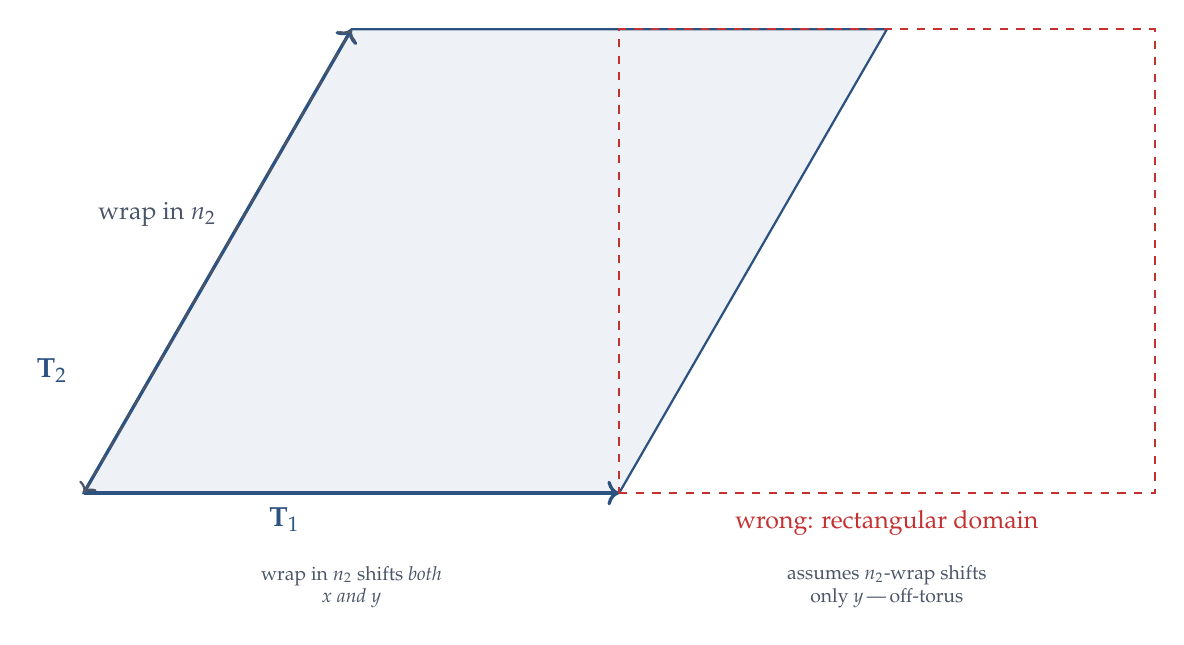
\begin{tikzpicture}[scale=0.85]
  \pgfmathsetmacro{\sq}{sqrt(3)}
  \pgfmathsetmacro{\Lmag}{4}
  \draw[thick, accent, fill=accent!8] (0,0) -- (\Lmag*2,0) -- (\Lmag*2 + \Lmag, \Lmag*\sq) -- (\Lmag, \Lmag*\sq) -- cycle;
  \node[accent] at (3, -0.4) {$\vT{1}$};
  \draw[->, very thick, accent] (0,0) -- (\Lmag*2, 0);
  \node[accent, anchor=south east] at (-0.1, 1.5) {$\vT{2}$};
  \draw[->, very thick, accent] (0,0) -- (\Lmag, \Lmag*\sq);
  \draw[<->, dashed, neutral, thick] (0, 0) -- (\Lmag, \Lmag*\sq);
  \node[neutral, font=\small] at (\Lmag*0.4-0.5, \Lmag*\sq*0.6) {wrap in $n_2$};
  \node[neutral, font=\scriptsize, align=center] at (4, -1.4) {wrap in $n_2$ shifts \emph{both}\\$x$ \emph{and} $y$};
  \draw[thick, bad, dashed] (8, 0) -- (8+\Lmag*2, 0) -- (8+\Lmag*2, \Lmag*\sq) -- (8, \Lmag*\sq) -- cycle;
  \node[bad, font=\small] at (8+\Lmag, -0.45) {wrong: rectangular domain};
  \node[neutral, font=\scriptsize, align=center] at (8+\Lmag, -1.4) {assumes $n_2$-wrap shifts\\only $y$\,---\,off-torus};
\end{tikzpicture}
\captionof{figure}{The correct triangular torus is the parallelogram
(left); Dipanjan's grid implicitly assumes the rectangular torus (right).
The two differ by the missing $x$-shift in the $n_2$-wrap.}
\end{center}

This is the Fourier-space expression of the geometric trap PI drew on
the board. He was right about ``PBC implementation wrong''; the
resolution is the sheared grid.

% ===============================================================
\section{Solving the dynamics: from $M(\vk)$ to $P(n_1, n_2, t)$}\label{sec:solving}

\subsection{Time evolution in Fourier space}\label{ssec:time-evol}

The Bloch-form master equation (\ref{eq:master_k}) is linear with
constant-in-time coefficients, so at each $\vk$:
\begin{equation}\label{eq:formal_evolve}
\bm{\Ptilde}(\vk, t) \;=\; e^{M(\vk)\, t}\, \bm{\Ptilde}(\vk, 0),
\qquad
\bm{\Ptilde}(\vk, t) \equiv \big(\Ptilde_0, \Ptilde_1, \ldots, \Ptilde_5\big)^{T}(\vk, t).
\end{equation}

\subsection{Initial condition}\label{ssec:ic}

A walker placed at the origin with a uniformly random initial director
has $P_m(n_1, n_2, 0) = \tfrac{1}{6}\, \delta_{n_1, 0}\, \delta_{n_2, 0}$.
Forward Fourier transform (\ref{eq:fft_pair}) gives
\begin{equation}\label{eq:psi0}
\Ptilde_m(\vk, 0) \;=\; \tfrac{1}{6}\, e^{\,i\vk\cdot\vr(0,0)} \;=\; \tfrac{1}{6} \quad \text{for all } m \text{ and all } \vk.
\end{equation}
Define the constant vector $\bm{\psi}_0 \equiv \tfrac{1}{6}(1, 1, 1, 1, 1, 1)^{T}$.

\subsection{Matrix exponential via eigendecomposition}\label{ssec:expm}

Diagonalise $M(\vk) = V(\vk)\, \Lambda(\vk)\, V(\vk)^{-1}$, where $\Lambda$
is diagonal with the six eigenvalues $\lambda_n(\vk)$. Then
\begin{equation}\label{eq:expm}
e^{M(\vk)\, t} \;=\; V(\vk)\, e^{\Lambda(\vk)\, t}\, V(\vk)^{-1},
\qquad \big[e^{\Lambda t}\big]_{nn'} = \delta_{nn'}\, e^{\lambda_n(\vk)\, t}.
\end{equation}
Combining (\ref{eq:formal_evolve}), (\ref{eq:psi0}), and (\ref{eq:expm}):
\begin{equation}\label{eq:ptilde_explicit}
\bm{\Ptilde}(\vk, t) \;=\; V(\vk) \cdot \mathrm{diag}\!\big(e^{\lambda_n(\vk) t}\big) \cdot V(\vk)^{-1} \cdot \bm{\psi}_0.
\end{equation}

\subsection{Marginal over director: total probability}\label{ssec:marginal}

The observable quantity (probability of finding the walker at site
$(n_1, n_2)$, summed over all director states) is
\begin{equation}\label{eq:Ptilde_total}
\Ptilde(\vk, t) \;\equiv\; \sum_{m=0}^{5} \Ptilde_m(\vk, t)
\;=\; \mathbf{1}^{T}\, V(\vk)\, \mathrm{diag}\!\big(e^{\lambda_n(\vk) t}\big)\, V(\vk)^{-1}\, \bm{\psi}_0,
\end{equation}
with $\mathbf{1} = (1, 1, 1, 1, 1, 1)^{T}$.

\subsection{Inverse Fourier transform onto the lattice}\label{ssec:invft-explicit}

Finally, applying the inverse Fourier sum (\ref{eq:ifft}) over the
$L^2$ sheared wavevectors:
\begin{correctbox}[The full chain in one line]
\begin{equation}\label{eq:full_chain}
P(n_1, n_2, t) \;=\; \frac{1}{L^2}\sum_{m_1, m_2 = 0}^{L-1}
  e^{\,-i \vk(m_1, m_2)\cdot \vr(n_1, n_2)} \;
  \underbrace{\mathbf{1}^{T} V(\vk)\, \mathrm{diag}(e^{\lambda_n(\vk) t})\, V(\vk)^{-1}\, \bm{\psi}_0}_{\Ptilde(\vk, t)}.
\end{equation}
\end{correctbox}
Using the integer-form identity (\ref{eq:k_dot_r_clean}),
$\vk(m_1, m_2) \cdot \vr(n_1, n_2) = 2\pi(m_1 n_1 + m_2 n_2)/L$, so the
exponential is a standard 2D DFT phase.

\paragraph{Implementation outline.}
\begin{enumerate}[label=(\arabic*),leftmargin=*,nosep]
\item For each $(m_1, m_2) \in \{0,\ldots,L-1\}^2$: build $\vk$ on the
  sheared grid (\ref{eq:k_shear}), assemble $M(\vk)$ from
  (\ref{eq:Mk_explicit}), call \texttt{numpy.linalg.eig} to get
  $(\lambda_n, V)$, and store $\Ptilde(\vk, t)$ from (\ref{eq:Ptilde_total}).
\item Inverse-FT once over the lattice via (\ref{eq:full_chain}) to get
  $P(n_1, n_2, t)$.
\end{enumerate}
This is what {\sf triangular\_jmvr\_corrected.py} does. Total cost:
$L^2$ eigendecompositions of $6\times 6$ matrices, plus one $L^2 \times L^2$
inverse FT.

% ===============================================================
\section{Verification}\label{sec:verification}

\begin{center}\small
\renewcommand{\arraystretch}{1.18}
\begin{tabular}{lrr}
\toprule
\textbf{case} & \textbf{RMS vs KMC} & \textbf{ratio to noise} \\
\midrule
\rowcolor{badfill!50} (1) rect grid + buggy $c_3$ (Dipanjan original) & $4.45 \times 10^{-4}$ & $105$ \\
\rowcolor{badfill!30} (2) rect grid + fixed $c_3$ & $4.59 \times 10^{-4}$ & $109$ \\
\rowcolor{badfill!30} (3) shear grid + buggy $c_3$ & $1.43 \times 10^{-4}$ & $34$ \\
\rowcolor{goodfill!60} \textbf{(4) shear grid + fixed $c_3$ (CORRECT)} & $\mathbf{3.43 \times 10^{-6}}$ & $\mathbf{0.81}$ \\
\bottomrule
\end{tabular}
\captionof{table}{Theory vs 100M-walker Fortran KMC at
$(\gamma, \epsilon, t, L) = (0.01, 0.15, 50, 30)$. MC noise floor
$\sqrt{P_{\rm max}/N} = 4.22\times10^{-6}$. Only case (4) reaches it.}
\end{center}

Either fix alone (cases 2, 3) leaves the theory off by 30--100$\times$
the noise. Both fixes are independent and both necessary.

% ===============================================================
\section{Summary}\label{sec:summary}

\begin{keyresult}[Two independent bugs in {\sf{rtp\_tl\_2.nb}} and Confinement~2021 draft Eq.~B11]
\begin{enumerate}[leftmargin=*]
\item \textbf{Wrong sign on $c_3$ chirality term.} Master equation for
  director $m=2$, after Fourier transform, gives
  \[
  c_3 \;=\; B(\vk) - 1 - \gamma \;-\; 2 i \epsilon \sin(a k_1 - b k_2),
  \]
  whereas the draft has $+$. Source: swap of forward NN displacement
  $\veps{2}$ with its opposite $\veps{5}$.

\item \textbf{Rectangular k-grid violates the triangular torus.}
  The notebook uses $k_x = \pi n_x/(aL),\; k_y = 2\pi n_y/(bL)$ on a
  $2L\times L$ grid. Odd-$n_x$ wavevectors fail
  $\vk \cdot \vT{2} \in 2\pi\mathbb{Z}$ and are off-torus.
  The correct sheared grid is
  $k_x = \pi m_1/(aL),\; k_y = \pi(2 m_2 - m_1)/(bL)$.
\end{enumerate}
\end{keyresult}

\noindent Either fix alone leaves the theory $\sim 30$--$100\times$ off
the KMC ground truth. Both together bring agreement to the MC noise
floor ($\text{RMS}_{\rm fix} = 3.4 \times 10^{-6}$ vs noise
$4.2 \times 10^{-6}$). The corrected $c_3$ should replace Eq.~B11 of the
Confinement~2021 draft, and the inverse Fourier in {\sf{rtp\_tl\_2.nb}}
should use the sheared grid (\ref{eq:k_shear}).

\appendix
\section{Connection to the JMVR 1D and 2D-square cases}\label{app:jmvr-other}

The JMVR paper's Appendix A treats the analogous 1D and 2D-square cases
explicitly. The Bloch matrices there are special cases of the general
framework above:

\paragraph{1D ($K = 2$ directors), derived in three lines.} States
$\pm$ on a 1D lattice. Director $+$ has $\veps{+} = +1$, director $-$
has $\veps{-} = -1 = -\veps{+}$ (the opposite-pair identity, with
$K/2 = 1$). The forward-backward pair for $m = +$ contributes
\[
(\tfrac{1}{2}+\epsilon)\,e^{ik} + (\tfrac{1}{2}-\epsilon)\,e^{-ik}
\;=\; \cos k + 2 i \epsilon \sin k.
\]
There are no sideways directions, so the bulk piece is just $\cos k$.
Diagonal entry: $M_{++} = \cos k - 1 - \gamma + 2 i \epsilon \sin k$.
Conjugation pairing $M_{--} = M_{++}^{*}$ (because
$\veps{-} = -\veps{+}$ and the rotation rate $\gamma$ between the two
states gives the off-diagonals). The matrix is
\[
M(k) = \begin{pmatrix} \cos k - 1 - \gamma + 2 i \epsilon \sin k & \gamma \\
\gamma & \cos k - 1 - \gamma - 2 i \epsilon \sin k \end{pmatrix},
\]
matching draft Eq.~A6. The same conjugation structure as in the
triangular case, just with one independent diagonal entry instead of
three.

\paragraph{2D square ($K = 4$ directors), stated without derivation.}
Same logic with NN displacements $\veps{0,1,2,3} = (\pm 1, 0), (0, \pm 1)$.
Forward rate $\tfrac{1}{4} + \epsilon$, backward $\tfrac{1}{4} - \epsilon$,
two sideways at $\tfrac{1}{4}$. The bulk piece, summing the two
opposite-pair cosines, is $\tfrac{1}{2}(\cos k_x + \cos k_y)$. The
diagonal entries are
\[
a = \tfrac{1}{2}(\cos k_x + \cos k_y) - 1 - \gamma + 2 i \epsilon \sin k_x,\quad
b = \tfrac{1}{2}(\cos k_x + \cos k_y) - 1 - \gamma + 2 i \epsilon \sin k_y,
\]
and the other two are $a^*, b^*$ (see draft Eq.~A17--A19; derivation is
identical in structure to Sec.~\ref{sec:bloch} above, just with
$K = 4$ and two independent diagonals instead of three).

The triangular case is the next member of the family: $K = 6$ directors,
three independent diagonals, and the third chirality is the one where
the sign got flipped in the draft.

\end{document}
